\chapter{Bases de Datos Temporales}  \label{cap:t}

\section{El dominio del tiempo}

% Intro
Estudiaremos ahora el problema de representar datos temporales y relaciones temporales entre datos,
ambos aspectos muy importantes de los fenómenos del mundo real.
La abilidad de modelar esta dimension temporal es esencial para aplicaciones informaticas como
econometría, bancos, control de inventario, contabilidad, leyes, registros médicos, sistemas de reservas de vuelos y muchas otras.

% DBs tradicionales: unico estado presente
Podemos introducir la idea de bases de datos temporales como una generalización a la siguiente intuición.
Una base de datos tradicional representa el estado del sistema en un momento específico: el presente.
En este sentido, a medida que la base de datos se modifica, las versiones anteriores se pierden.
Los datos desactualizados son borrados de la base de datos.
Surge entonces la problemática de las aplicaciones para las cuales nos sería útil conservar estos estados anteriores
y las relaciones entre sus datos.

% Recorrido del capítulo
%TODO: mejorar con recorrido de capitulo
Para poder plantear una implementación para una base de datos temporal es necesario comprender cómo se comporta y cómo se observa el tiempo.
A lo largo de este capitulo exploraremos algunos modelos y representaciones del mismo junto con
las elecciones para poder plantear una solución a los problemas temporales.

\subsection{La estructura del tiempo}

% Something something empieza teórico
En el cápitulo anterior vimos como la investigación de bases de datos espaciales se vio motivada por
la necesidad práctica de mejorar el manejo de datos de los sistemas GIS.
Las bases de datos temporales por su parte, fueron fuertemente impactadas por
la investigación previa en lógica temporal de los años 70 \cite{temporal:status:directions}.
Los trabajos fundacionales de la lógica temporal han dividido el estudio del tiempo en dos modelos estructurales principales:
\textbf{lineal} y \textbf{ramificado} \cite{temporal:snodgrass}.
Comenzaremos entonces por estudiar estos modelos y luego mencionaremos brevemente otras posibilidades.

\subsubsection{Modelo Lineal}

Es el modelo más simple, donde el tiempo avanza del pasado al futuro de forma ordenada formando así una secuencia
tal y como se ve en la figura \ref{fig:linear-time-model}.

\begin{figure}
    \centering
    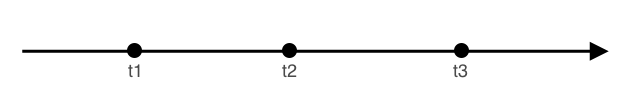
\includegraphics[scale=0.5]{fig-linear-time.png}
    \caption{Ejemplo de modelo lineal del tiempo}
    \label{fig:linear-time-model}
\end{figure}

Generalmente esta estructura es útil para mantener información histórica centrada en eventos del pasado.
Por ejemplo: registros de transacciones de un banco, sistemas de control de inventario, etc.

\subsubsection{Modelo ramificado}

A diferencia del modelo anterior, el tiempo se presenta dos formas:
se extiende de forma lineal desde el pasado hacia el presente formando una secuencia.
Podemos visualizar este modelo en la figura \ref{fig:branched-time-model}
y se ramifica del presente al futuro creando un árbol con raíz en el \textit{ahora} cuyas ramas se extienden hacia el futuro.

\begin{figure}
    \centering
    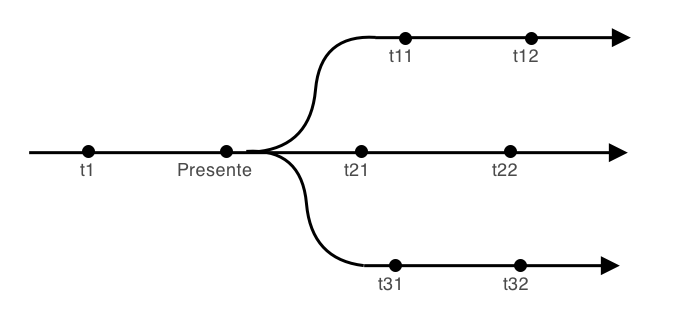
\includegraphics[scale=0.5]{fig-branched-time.png}
    \caption{Ejemplo de modelo ramificado del tiempo}
    \label{fig:branched-time-model}
\end{figure}

A esta forma de organizar el tiempo también se la conoce con el nombre de “modelo de los posibles futuros”.
Debido a sus características es útil para representar y trabajar con información predicativa.

\subsubsection{Elección entre estructuras temporales}

Los modelos más generales del tiempo en la lógica temporal representan el tiempo como un conjunto arbitrario
que cumple con la restricción de ser un \textit{orden parcial}.
Otros axiomas introducen otros modelos más refinados del tiempo.
Por ejemplo: el tiempo lineal puede ser simplificado agregando un axioma imponiendo un \textit{orden total} en este conjunto.
Un modelo recurrente, por otra parte, puede trabajarse con un \textit{modelo cíclico} del tiempo.

A lo largo de este trabajo se utilizará un modelo lineal del tiempo ya que es el más sencillo
y brinda todas las característicasnecesarias en las bases de datos temporales.

\subsection{La densidad del tiempo}

%TODO citas aca cuando tenga las citas del pelotudo de Snodgrass
Siguiendo con el modelo lineal, la densidad del tiempo puede variar en la línea.
Esta se puede clasificar en dos grupos: \textit{discretos} y \textit{densos}.

\subsubsection{Modelos Discretos}

Estas representaciones son isomorfas a los números naturales, lo que implica que cada punto en el tiempo tiene un único sucesor. Cada número natural corresponde a una unidad no descomponible de tiempo de duración arbitraria. Estas reciben el nombre de \textit{chronons}.  

\subsubsection{Modelos Densos}

Por su parte, los modelos densos, presentan dos variaciones: pueden ser isomorfos tanto a los números racionales como a los reales. Como consecuencia, dados dos momentos cualquiera en el tiempo existe otro momento entre ellos.

Los modelos isomorfos a los reales también son conocidos como continuos. En ellos cada número real corresponde a un punto en el tiempo. 




\subsubsection{\textit{Chronons} y la elección del modelo de densidad}
Un \textbf{chronon} es la duración de tiempo más pequeña que puede ser representada. Cabe destacar que no se trata de un punto sino un segmento en la línea del tiempo.

A pesar de que el tiempo en sí mismo suele ser percibido como algo continuo, la mayoría de las propuestas para agregar una dimensión temporal a los modelos de datos relacionales están basados en un modelo discreto del tiempo. Existen varias razones para esta elección entre las que se destacan cuatro:

\begin{itemize}
    \item Las medidas del tiempo son inherentemente imprecisas. Los instrumentos de medición temporal invariablemente reportan la ocurrencia de eventos en términos de chronons. No en “puntos” de tiempo. Por lo tanto, incluso los eventos así llamados “instantáneos” pueden ser medidos como si hubieran ocurrido durante un chronon, en el mejor de los casos.
    \item Las referencias del lenguaje más naturales del tiempo son compatibles con el modelo discreto del tiempo. Por ejemplo, cuando se dice que un evento ocurrió a las 4:30 PM, en realidad no se hace referencia a que el evento ocurrió en el “punto” del tiempo asociado a las 4:302 PM, sino a algún momento en el chronon asociado con las 4:30 PM aunque exista una variación de uno o dos minutos.
    \item Los conceptos de chronon y de intervalo permiten modelar naturalmente eventos que no son instantáneos pero que tienen duración.
    \item Cualquier implementación de un modelo de datos con dimensión temporal tendrá la necesidad de codificar el tiempo de forma discreta, es decir, que es inevitable discretizar el tiempo en algún punto.
    
\end{itemize}